\subsection{色反転処理の実装方式と実行時間}

課題 4 の色反転は、numpy のベクトル演算 {\tt 255 - frame} により
フレーム全体を一括で計算する方式を採用した。この設計選択が実行時間の
面でどの程度有利かを定量化するため、追加実験(実験ソースは付録の
{\tt exp03\_invert\_timing.py})として、(1) 実装方式 4 種の 1 フレーム
あたり実行時間の比較、(2) 画素数を変えたときのスケーリング特性の計測、
(3) 動画全体の処理時間に占める反転処理の割合の計測を行った。
計測対象は Cat - 66004.mp4(1280$\times$720、294 フレーム、29.97 fps)で
ある。時間計測には {\tt timeit} を用い、計測前に 3 回の空実行で
キャッシュと遅延初期化の影響を除いたうえで、1 セットの総時間が約
0.2 秒になるよう 1 セットあたりの実行回数({\tt number})を自動決定し、
7 セット({\tt repeat=7})の 1 回あたり時間の中央値を代表値とした。実行環境は表 \ref{tab:env} と
同一(Apple Silicon、Python 3.13.2、numpy 2.4.4、OpenCV 4.12.0)である。

なお、OpenCV の {\tt cv2.bitwise\_not()} は本課題の制約により提出
プログラムでは使用できない。本実験では提出プログラムには一切含めず、
最適化された既製実装がどの程度の速度を出すかを知るための
速度基準としてのみ参考計測した。

\subsubsection{比較した実装方式と計測条件}

色反転は、8 bit 画像の各画素値 $p$ に対して

\begin{equation}\label{eq:b3-invert}
p' = 255 - p
\end{equation}

を全画素・全チャネルに適用する処理である。式 \ref{eq:b3-invert} の
計算内容は同一のまま、「どの層でループを回すか」だけが異なる次の
4 方式を比較した。

\begin{enumerate}
\item 方式 (a): {\tt 255 - frame}。numpy のブロードキャストにより
      配列全体を一括計算する。提出プログラムの採用手法であり、
      出力用の新しい配列が毎回確保される。
\item 方式 (b): {\tt np.subtract(255, frame, out=buf)}。計算内容は
      方式 (a) と同じだが、事前に確保した出力バッファ {\tt buf} を
      再利用することで、呼び出しごとのメモリ確保を省く。
\item 方式 (c): Python の 3 重ループ。{\tt for} 文で行・列・チャネルを
      走査し、画素成分ごとに式 \ref{eq:b3-invert} を計算する。
      フルサイズでは時間がかかりすぎるため 160$\times$90 に縮小した
      フレームで実測し、処理量が画素数に比例するとみなして
      式 \ref{eq:b3-extrapolate} でフルサイズへ換算した
      (この比例仮定の妥当性は後述のスケーリング実験で確認する)。
\item 方式 (d): {\tt cv2.bitwise\_not(frame)}。uint8 のビット反転
      $\overline{p}=255-p$ を利用した OpenCV の既製実装である
      (前述のとおり参考計測のみ)。
\end{enumerate}

\begin{equation}\label{eq:b3-extrapolate}
T_{1280\times 720} = T_{160\times 90} \times
\frac{1280 \times 720}{160 \times 90} = 64\, T_{160\times 90}
\end{equation}

計測に先立ち、4 方式の出力を {\tt np.array\_equal} で比較し、
すべて一致すること(方式 (c) は 160$\times$90 で確認)を確認した。
したがって以降の比較は「同一の結果を返す実装同士」の純粋な
実行時間比較である。

\subsubsection{ループ実装とベクトル化実装の比較}

1 フレーム(1280$\times$720$\times$3、uint8)に対する各方式の実行時間を
表 \ref{tab:b3-methods} に、その対数軸での比較を図 \ref{fig:b3-methods} に
示す。

\begin{table}[htbp]
\centering
\caption{色反転の実装方式別の 1 フレームあたり実行時間(7 回計測の中央値・最小・最大)}
\label{tab:b3-methods}
\begin{tabular}{llrrrl}
\hline
方式 & 計測サイズ & 中央値 [ms] & 最小 [ms] & 最大 [ms] & 備考 \\
\hline
(a) {\tt 255 - frame} & 1280$\times$720 & 2.216 & 0.691 & 2.525 & 採用手法 \\
(b) {\tt np.subtract(out=)} & 1280$\times$720 & 0.790 & 0.296 & 1.467 & バッファ再利用 \\
(c) Python 3 重ループ & 160$\times$90 & 39.98 & 20.97 & 87.62 & 実測 \\
(c) Python 3 重ループ & 1280$\times$720 & 2558.9 & 1342.1 & 5607.5 & 64 倍換算値 \\
(d) {\tt cv2.bitwise\_not} & 1280$\times$720 & 1.332 & 0.816 & 3.283 & 参考(使用禁止) \\
\hline
\end{tabular}
\end{table}

\begin{figure}[htbp]
\centering
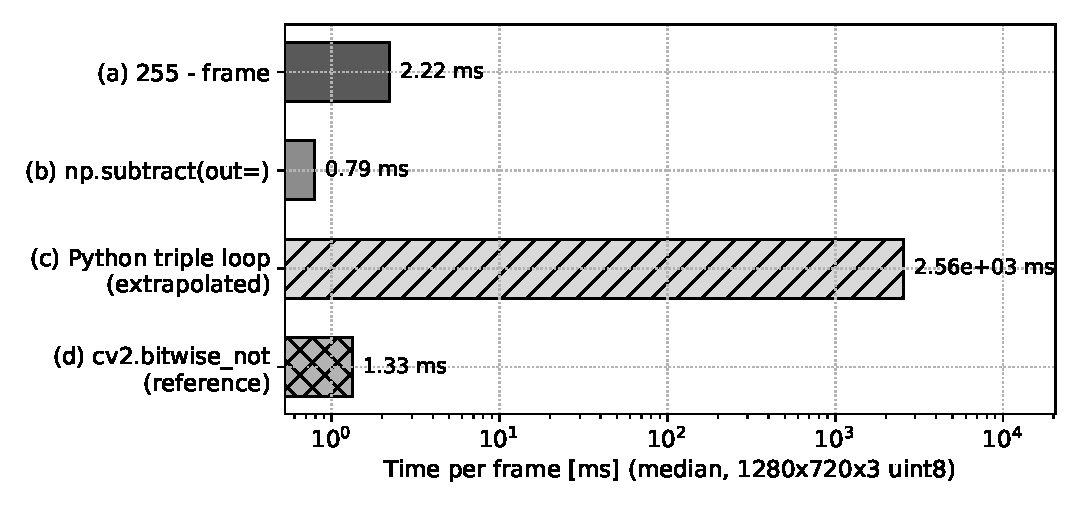
\includegraphics[width=0.9\linewidth]{../experiments/figures/exp03_methods.pdf}
\caption{実装方式別の 1 フレームあたり実行時間(横軸は対数)。方式 (c) は
160$\times$90 の実測値を式 \ref{eq:b3-extrapolate} で換算した推定値である。}
\label{fig:b3-methods}
\end{figure}

表 \ref{tab:b3-methods} のとおり、Python 3 重ループ(換算値 2559 ms)は
採用手法の {\tt 255 - frame}(2.216 ms)の約 1150 倍遅い。
1 画素成分あたりに直すと、3 重ループは
$39.98\ \mathrm{ms} / (160 \times 90 \times 3) \approx 0.93\ \mu\mathrm{s}$、
ベクトル演算は
$2.216\ \mathrm{ms} / (1280 \times 720 \times 3) \approx 0.80\ \mathrm{ns}$
であり、3 桁の差がある。両者は式 \ref{eq:b3-invert} という同一の計算を
しているから、この差は減算そのものではなく、画素成分ごとに発生する
Python インタープリタの処理(バイトコードの解釈、配列要素の取り出しと
uint8 スカラーオブジェクトの生成、ループ変数の管理)に費やされている。
numpy のベクトル演算では、この要素ごとの解釈実行が配列全体で 1 回の
コンパイル済み C ループに置き換わる。配列全体への一括操作
(ベクトル化)が配列プログラミングの性能の中心であることは
NumPy の設計論文 \cite{b3-numpy} でも述べられており、さらに numpy は
実行時に CPU の SIMD 命令セットを検出して最適化済みカーネルを選択する
機構を持つ \cite{b3-simd}。本実験の 3 桁の速度差は、これらの効果の
実測値である。

換算値であるフレーム 1 枚 2.56 秒という時間は、動画の再生間隔
$1/29.97 \approx 33.4$ ms の約 77 倍であり、3 重ループ実装では
1 フレームの反転すら再生速度に間に合わない。一方、採用手法の
2.216 ms は再生間隔の 6.6 \% にすぎない。課題の制約
({\tt cv2.bitwise\_not()} 禁止)の下で numpy のベクトル演算を
選択したことは、実行時間の観点から妥当であったといえる。

\subsubsection{メモリ確保の影響と in-place 版・既製実装との比較}

表 \ref{tab:b3-methods} では、出力バッファを再利用する方式 (b) が
0.790 ms と、採用手法 (a) の 2.81 倍速い。両者の計算内容は同一で、
異なるのは呼び出しごとに約 2.76 MB
($1280 \times 720 \times 3$ バイト)の出力配列を新規確保するか
どうかだけである。したがってこの差は、大きな配列のメモリ確保・
初期ページアクセスのコストが減算本体と同程度以上に大きいことを
示している。同じことは計測の変動幅にも現れており、方式 (a) の
1 回あたり時間は最小 0.691 ms から最大 2.525 ms まで約 3.7 倍の幅を
持つ。後述の表 \ref{tab:b3-scaling} の同一解像度(1280$\times$720)では
方式 (a) が 0.691 ms と計測されており、これはメモリアロケータの状態
(解放済みページが再利用できるか)によって同一処理の時間が数倍変わる
ためと考えられる。

参考計測した {\tt cv2.bitwise\_not}(1.332 ms)は方式 (a) の
1.66 倍速いが、方式 (b) より遅い。また表 \ref{tab:b3-scaling} の
同一解像度では逆に方式 (a) が方式 (d) の 2.7 倍速く、両者の大小関係は
計測区間によって入れ替わる。すなわち方式 (a)・(b)・(d) の差は
いずれもメモリ確保やアロケータ状態に起因する変動(数倍)の範囲に
あり、3 桁の差を持つループ実装との比較とは質的に異なる。この結果から、
本課題の規模では「ベクトル化されているか否か」が支配的であり、
使用が禁止されている {\tt cv2.bitwise\_not} を使えないことによる
性能上の不利は実質的にないと結論できる。

なお、毎フレームの処理時間で概算すると、方式 (a) は入出力あわせて
約 5.53 MB のデータを 2.216 ms で処理しており、実効メモリスループットは
約 2.5 GB/s、方式 (b) では約 7.0 GB/s に達する。処理が演算律速では
なくメモリ律速に近いことも、メモリ確保の削減(方式 (b))が
そのまま高速化につながる理由である。

\subsubsection{画素数に対するスケーリング}

色反転の処理量は画素数 $N$ に比例するはずである。これを確認するため、
解像度を 160$\times$90 から 2560$\times$1440 まで 4 倍刻みで変えて
方式 (a) と方式 (d) の時間を計測した。処理時間が

\begin{equation}\label{eq:b3-power}
T(N) = c\,N^{\alpha}
\qquad \Longleftrightarrow \qquad
\log_{10} T = \alpha \log_{10} N + \log_{10} c
\end{equation}

に従うとすれば、両対数プロットの傾きが指数 $\alpha$ を与える。
結果を表 \ref{tab:b3-scaling} と図 \ref{fig:b3-scaling} に示す。

\begin{table}[htbp]
\centering
\caption{解像度(画素数)に対する 1 フレームあたり実行時間の変化(中央値)}
\label{tab:b3-scaling}
\begin{tabular}{rrrr}
\hline
解像度 & 画素数 & (a) {\tt 255 - frame} [ms] & (d) {\tt cv2.bitwise\_not} [ms] \\
\hline
160$\times$90 & 14400 & 0.0210 & 0.0174 \\
320$\times$180 & 57600 & 0.0793 & 0.0852 \\
640$\times$360 & 230400 & 0.2502 & 0.4770 \\
1280$\times$720 & 921600 & 0.6909 & 1.8703 \\
2560$\times$1440 & 3686400 & 7.4146 & 4.0265 \\
\hline
\end{tabular}
\end{table}

\begin{figure}[htbp]
\centering
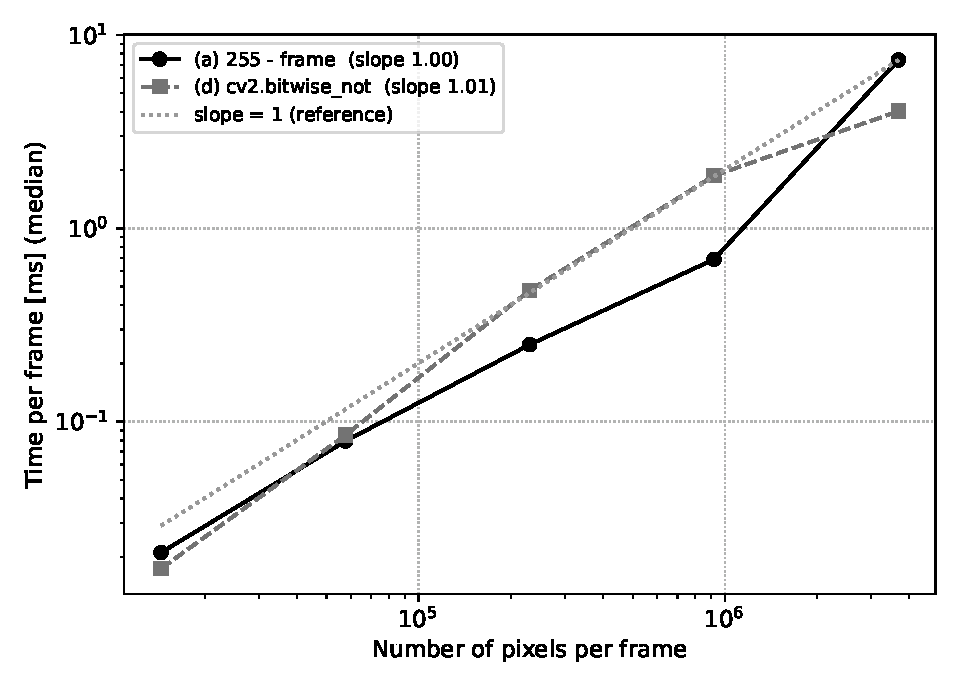
\includegraphics[width=0.75\linewidth]{../experiments/figures/exp03_scaling.pdf}
\caption{画素数に対する色反転時間の両対数プロット。点線は傾き 1
(時間 $\propto$ 画素数)の基準線である。}
\label{fig:b3-scaling}
\end{figure}

最小二乗法による式 \ref{eq:b3-power} の傾きは、方式 (a) が
$\alpha = 1.002$、方式 (d) が $\alpha = 1.009$ であり、いずれも
ほぼ 1 に一致した。図 \ref{fig:b3-scaling} でも両系列は傾き 1 の
基準線とほぼ平行である。すなわち色反転の実行時間は画素数に対して
線形($O(N)$)であり、方式 (c) の換算(式 \ref{eq:b3-extrapolate})で
用いた「処理量は画素数に比例する」という仮定はベクトル化実装に
おいて成立している。また、画素数が 256 倍(14400 → 3686400)変わると
時間は約 350 倍変わるのに対し、同一画素数での方式 (a) と (d) の差は
最大でも 2.7 倍にとどまる。解像度の選択が実装方式の選択より
実行時間への影響がはるかに大きいことが分かる。

\subsubsection{動画処理全体に占める反転処理の割合}

課題 4 の実処理は「読み込み → 反転 → 0.3 倍リサイズ → 書き出し」の
繰り返しである。{\tt time.perf\_counter} で 4 区間を分けて累積計測した
結果を表 \ref{tab:b3-pipeline} と図 \ref{fig:b3-pipeline} に示す。

\begin{table}[htbp]
\centering
\caption{動画全体(294 フレーム)の処理時間の内訳}
\label{tab:b3-pipeline}
\begin{tabular}{lrrr}
\hline
区間 & 合計 [s] & 1 フレーム平均 [ms] & 割合 [\%] \\
\hline
読み込み({\tt cap.read}) & 5.292 & 18.00 & 67.7 \\
反転({\tt 255 - frame}) & 0.477 & 1.62 & 6.1 \\
リサイズ({\tt cv2.resize}) & 0.873 & 2.97 & 11.2 \\
書き出し({\tt writer.write}) & 1.172 & 3.99 & 15.0 \\
\hline
4 区間合計 & 7.815 & 26.58 & 100.0 \\
\hline
\end{tabular}
\end{table}

\begin{figure}[htbp]
\centering
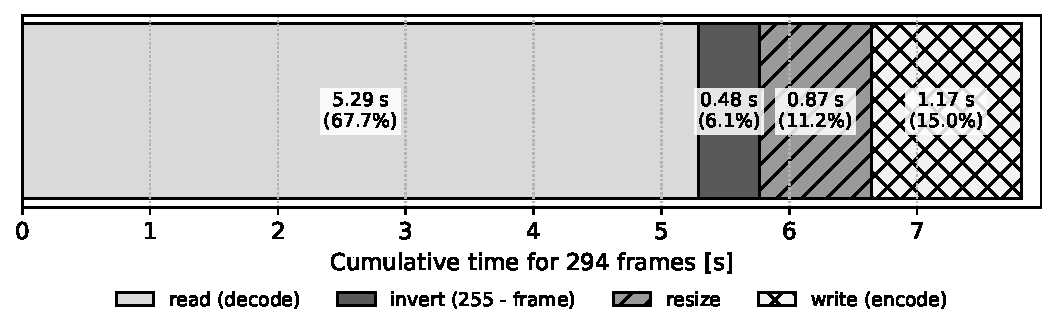
\includegraphics[width=0.95\linewidth]{../experiments/figures/exp03_pipeline.pdf}
\caption{動画全体(294 フレーム)の処理時間の内訳(積み上げ棒)。}
\label{fig:b3-pipeline}
\end{figure}

表 \ref{tab:b3-pipeline} のとおり、全体 7.81 秒のうち 67.7 \% は
動画のデコード({\tt cap.read})が占め、反転処理はわずか 6.1 \%
(0.477 秒)である。1 フレームあたりの合計 26.6 ms は再生間隔
33.4 ms を下回っており、採用実装は実時間より速く動画を変換できる。

この内訳は 2 つの結論を与える。第一に、仮に反転処理を方式 (c) の
3 重ループで実装した場合、反転だけで
$2.559\ \mathrm{s} \times 294 \approx 752$ 秒を要し、全体の処理時間は
約 7.8 秒から約 760 秒へと 97 倍に悪化すると見積もられる。ベクトル化の
採否は、この処理系全体の実用性を左右する決定的な要因である。第二に、
逆に反転処理をこれ以上高速化しても(たとえば方式 (b) や方式 (d) に
置き換えて反転時間を 0 に近づけても)全体は最大 6.1 \% しか短縮
されない。全体の律速はデコードであるから、さらなる高速化を図るなら
反転の実装ではなく、フレームの読み飛ばしやデコード解像度の削減など
入力側の工夫が必要である。採用した {\tt 255 - frame} は、課題の制約を
満たしつつ、処理全体の中でボトルネックにならない十分な速度を持つと
結論できる。
